\documentclass{applemlr}

\usepackage{amsmath, amssymb}
\usepackage{graphicx}
\usepackage{booktabs}
\usepackage{tabularx}
\usepackage{array}
\usepackage{enumitem}
\usepackage{listings}
\usepackage{caption}
\usepackage{float}

\setcounter{tocdepth}{2}
\setlist[itemize]{leftmargin=*, itemsep=0.4em}
\setlist[enumerate]{leftmargin=*, itemsep=0.4em}
\newcolumntype{Y}{>{\centering\arraybackslash}X}

\definecolor{listingbg}{gray}{0.95}
\definecolor{listingborder}{HTML}{D0D3D4}
\definecolor{listingcomment}{HTML}{5E8050}
\definecolor{listingkeyword}{HTML}{007AFF}

\lstdefinestyle{aiproject}{
  backgroundcolor=\color{listingbg},
  frame=single,
  framerule=0.4pt,
  rulecolor=\color{listingborder},
  basicstyle=\ttfamily\footnotesize,
  keywordstyle=\color{listingkeyword}\bfseries,
  commentstyle=\color{listingcomment},
  numbers=left,
  numberstyle=\scriptsize\color{listingkeyword},
  stepnumber=1,
  numbersep=6pt,
  breaklines=true,
  columns=fullflexible,
  captionpos=b,
  keepspaces=true
}


\usepackage{xcolor}       % 用于颜色定义
\usepackage[most]{tcolorbox} % 引入 tcolorbox 宏包

\newtcbox{\code}{
  nobeforeafter, % 确保它是一个行内命令
  colback=black!10, % 背景颜色 (10%的黑色，即浅灰色)
  colframe=black!60, % 边框颜色 (60%的黑色)
  boxrule=0.5pt,    % 边框粗细
  arc=2pt,          % 圆角大小
  boxsep=0pt,       % 内部文字与边框的间距
  left=3pt, right=3pt, top=2pt, bottom=2pt, % 分别设置四个方向的间距
  % raise=1.5pt, % 稍微向上调整盒子位置，让它和文本对齐更好看
  fontupper=\ttfamily % 盒子内的文字使用打字机字体
}




\title{AI 智能衣柜助手项目报告}

\author{武昂达}
\author{刘景鲁豫}
\author{姚文熙}
\affiliation{上海交通大学自动化与感知学院}

\metadata[课程信息]{人工智能算法实践}
\metadata[提交日期]{2026 年 6 月}

\abstract{
本文节选 AI 智能衣柜助手项目报告中的系统总体设计与方法设计部分。项目围绕个性化穿搭推荐任务，构建了一个本地 Web 原型系统，结合用户资料、用户衣柜、历史偏好和 RAG 穿搭样例，通过千问完成需求解析与穿搭生成，并通过前端规则校验和万相图像生成实现可解释、可视化的穿搭推荐流程。
}

\begin{document}

\maketitle

\tableofcontents
\newpage

\section{引言}
\label{sec:intro}

对于现在的大学生而言，日常生活中有许多看似轻松不要紧，实际研究起来却耗费时间和精力的事情，穿搭就是其中的一个典型例子。
每天上课、实验、社团、面试或出游等等，不同场合下的衣着风格有不同要求；
但现实中，许多同学往往因为时间紧、经验不足，或是懒得反复搭配，最后长期停留在几套固定组合上。
例如许多男同学夏天习惯上身短袖加条黑短裤，冬天则是羽绒服加条长裤，不用太过考虑，一套就能管一周。
这样的选择虽然足够方便，但却很难体现个人风格，无形中让生活少了一些精致，还容易让衣柜中已有的衣物利用率变低。
而随着大语言模型与多模态生成技术的发展，AI 工具展现出的能力已经逐渐从单纯回答问题"进化"为共同参与决策。
因此，我们想到搭建一个 AI 衣柜助手，让它来帮助我们参谋每天应该穿些什么。

我们认为穿搭推荐并不只是一个简单的文本生成问题，
直接向大模型询问"今天穿什么"虽然能够得到一些建议，但这类建议往往比较泛泛，甚至会推荐用户根本没有的衣服。
一个真正可用、可靠的 AI 智能衣柜助手，需要同时理解用户的基本信息、场合需求、风格偏好、已有衣物以及历史反馈，并在这些约束下给出具体、可执行的搭配方案。
因此，我们希望将大语言模型从一次性的聊天工具，进一步构建成一个\textbf{面向日常穿搭决策的个性化 AI Agent。}

基于这个目标，我们\textbf{设计并实现了 AIWardrobe ———— 一个基于 Qwen 大模型的 AI 智能衣柜穿搭助手。}
这个助手支持用户创建个人档案，维护自己的衣柜，并通过自然语言输入当天的场景、心情、天气或风格需求。
为了避免推荐结果脱离现实，助手在生成穿搭方案前会结合用户衣柜信息，并利用人工收集和描述的 150 余条穿搭案例构建参考案例库，通过语义向量检索找到与当前需求相近的搭配风格。
与此同时，系统还会从用户对话中抽取长期偏好，例如喜欢的颜色、版型、风格以及明确不喜欢的元素，使后续推荐能够逐渐贴近用户个人习惯。

从技术实现上来看，我们的项目搭建了"需求解析—安全审核—案例检索—衣柜约束—方案生成—可视化展示—偏好更新"的完整链路。
前端负责用户信息录入、衣柜编辑、对话交互和结果展示，后端负责模型调用、RAG 检索、Prompt 组织、数据存储与异常兜底。
穿搭助手不仅生成三套文字化穿搭建议，还提供参考案例证据和虚拟上身效果，使用户能够更直观地判断推荐是否符合自己的需求。
因此，相较于单纯的大模型问答，\textbf{我们的穿搭助手更强调穿搭的系统性、个性化和可落地性。}

我们的报告将围绕 AIWardrobe 助手的设计与实现展开说明。
首先，我们将介绍相关工作与项目使用的数据来源；
之后，我们会阐述系统架构、RAG 检索机制、用户偏好记忆、衣柜约束与多模态生成流程等链路流程涉及到的结构与技术；
最后通过具体实验分析助手在穿搭推荐、个性化适配和安全可靠性方面的表现，并对我们的项目进行进一步发展的展望。


\section{相关工作}
\label{sec:related-works}

本项目涉及的相关工作主要可以从四个方面展开：
个性化穿搭推荐、检索增强生成、大语言模型智能体与个性化记忆、多模态图像生成与虚拟上身。
这些方向分别对应项目中的推荐方案、参考案例检索、用户偏好记忆和上身可视化模块。

\subsection{个性化穿搭推荐}

穿搭推荐不同于普通商品推荐，它不仅要判断用户是否喜欢某件单品，还要考虑多件衣物之间的组合关系。
Han et al. 提出利用序列模型学习服装单品之间的兼容性，将一套 outfit 看作多个 fashion item 组成的序列，
从而判断整体搭配是否合理 \citep{han2017learning}。
后续也有工作使用 Transformer 建模 outfit 中不同单品的关系，
例如 Sarkar et al. 的 OutfitTransformer 就用于学习整套穿搭的表示，
从而支持后续服装兼容性判断和推荐任务 \citep{sarkar2023outfittransformer}。
这些研究说明，穿搭推荐的重点并不是简单推荐单件衣服，而是理解颜色、版型、风格、材质和场景之间的组合关系。

不过，现实中的穿搭推荐还需要考虑"可穿性"。如果系统推荐了用户衣柜中不存在的衣服，即使风格上合理，也难以真正落地。
因此，我们的项目在生成穿搭方案时加入了用户衣柜约束，使模型的推荐结果尽量围绕用户已有衣物展开。
这也是本项目区别于普通聊天式穿搭模型的重要特点。

\subsection{检索增强生成 (RAG)}

检索增强生成是一类将外部知识检索与大模型生成相结合的方法。
Lewis et al. 提出的 RAG 框架将参数化生成模型与非参数化知识索引结合，
在生成答案前先检索相关文档，再基于检索结果进行回答 \citep{lewis2020retrieval}。
这一思想能够在一定程度上减少模型幻觉，同时提升生成结果与具体任务之间的相关性。
我们意识到用户的衣柜与模型返回的穿搭结果也应该具有这种强相关性，因而这启发我们在项目中运用 RAG 技术让大模型生成穿搭。

在我们的项目中，RAG 并不是用于检索百科知识，而是用于检索穿搭参考案例。
在调用模型前，我们人工整理了 150 余条社交媒体穿搭案例，并为每条案例标注了风格、颜色、场景和搭配简介。
当用户输入穿搭需求后，系统会根据语义向量检索相似案例，并将这些案例作为大模型生成穿搭方案的参考。
通过这种方法，可以让模型的推荐结果更具体、更"有人味"，也更接近真实穿搭场景。

\subsection{大语言模型智能体与个性化记忆}

近年来，大语言模型逐渐从单轮问答工具发展为能够调用工具、保存记忆并执行多步骤任务的智能系统。
Park et al. 提出的 Generative Agents 展示了如何为语言模型代理构建记忆、反思和规划机制，
使其能够在虚拟环境中表现出连续的行为 \citep{park2023generative}。
这一思路启发我们将穿搭助手设计为一个具有状态和记忆的个性化 Agent，而不是一次性的文本生成器。

对于我们的项目而言，用户的历史偏好非常重要。
若用户曾表达"不喜欢高跟鞋""喜欢宽松版型"或"偏好冷色系"等个性化偏好，那么这些信息都应该影响后续推荐。
因此，助手应当主动从对话中抽取 likes、dislikes 和 contextual preferences 等结构化偏好，并在后续生成中作为约束使用。
同时，为了避免用户输入中含有越权请求或有 prompt injection 等影响模型的行为，我们也在需求解析阶段加入了安全审核。

\subsection{多模态生成与虚拟上身}

穿搭推荐天然具有视觉属性。单纯的文字建议虽然能够说明"上衣搭配什么裤子"，但用户往往仍然需要在脑中想象整体效果。
这就会为用户带来额外的思考成本，尤其对于不熟悉穿搭的人来说，文字描述和真实上身效果之间仍然存在距离。
因此，近年来多模态图像生成、虚拟试穿和人物图像编辑技术也逐渐被应用到服装展示和搭配预览中。

虚拟试穿任务的目标是在保留人物身份、姿态和体型的同时，将目标服装自然地迁移到人物图像上。
Zhu et al. 的 TryOnDiffusion 及同类工作表明，扩散模型能够在服装保真度和人物图像自然度之间取得较好的平衡，
这为服装展示和试穿预览提供了新的技术路径 \citep{zhu2023tryondiffusion}。
虽然本项目中的穿搭可视化模块并不追求精确的服装物理仿真，但它可以给用户提供一个直观的视觉参考。
用户在查看三套穿搭方案后，可以进一步观察对应的虚拟穿搭效果图，从整体比例、颜色关系和风格氛围上判断推荐是否符合预期。

总体而言，我们的 AIWardrobe 并不是简单套用某一个已有模型，而是综合了穿搭推荐、RAG 检索、
个性化记忆和多模态生成等多个方向技术的穿搭 Agent。
我们项目的重点不在于提出一个新的基础模型或推荐算法，
而在于\textbf{将大模型已有的强大能力通过技术手段组织成一个完整、可交互、可落地的日常穿搭决策智能体。}

\section{数据构建}
\label{sec:data}

本项目的数据构建工作主要围绕两条主线展开：一是面向用户的个性化数据，包括用户档案、衣柜信息和历史偏好记忆；二是面向模型的参考样例数据，包括穿搭案例及其向量索引。两类数据在系统中承担不同角色：用户侧数据驱动个性化推荐，样例侧数据提供风格与场景参考。

\subsection{穿搭样例收集与描述}

为了使模型生成的穿搭方案不脱离实际审美，三位同学事先从社交媒体穿搭内容中收集了 150 余张穿搭案例图片，案例来源以中文社交平台中的高质量穿搭分享为主，涵盖了不同性别、季节、场合和风格的搭配。

每一条样例除了保留原始图片外，我们还额外进行了人工标注。标注信息以自然语言描述和结构化标签两种形式记录在 \code{Description\_example.json} 中。如图~\ref{fig:data-build} 所示，样例数据的构建流程包括图片收集、人工标注描述与标签、文本拼接和向量化四个步骤。

每条样例描述遵循统一格式，包含以下字段：衣物描述（逐件说明上装、下装、鞋包等单品）、性别、适宜季节、适宜场合、穿搭风格、风格关键词、主要色彩和可见单品列表。同时，每条样例还附带结构化 \code{tags}，包含 \code{gender}、\code{season}、\code{occasion}、\code{style} 和 \code{colors} 五个维度，每个维度以列表形式保存，便于后续检索和统计。

\begin{figure}[ht]
  \centering
  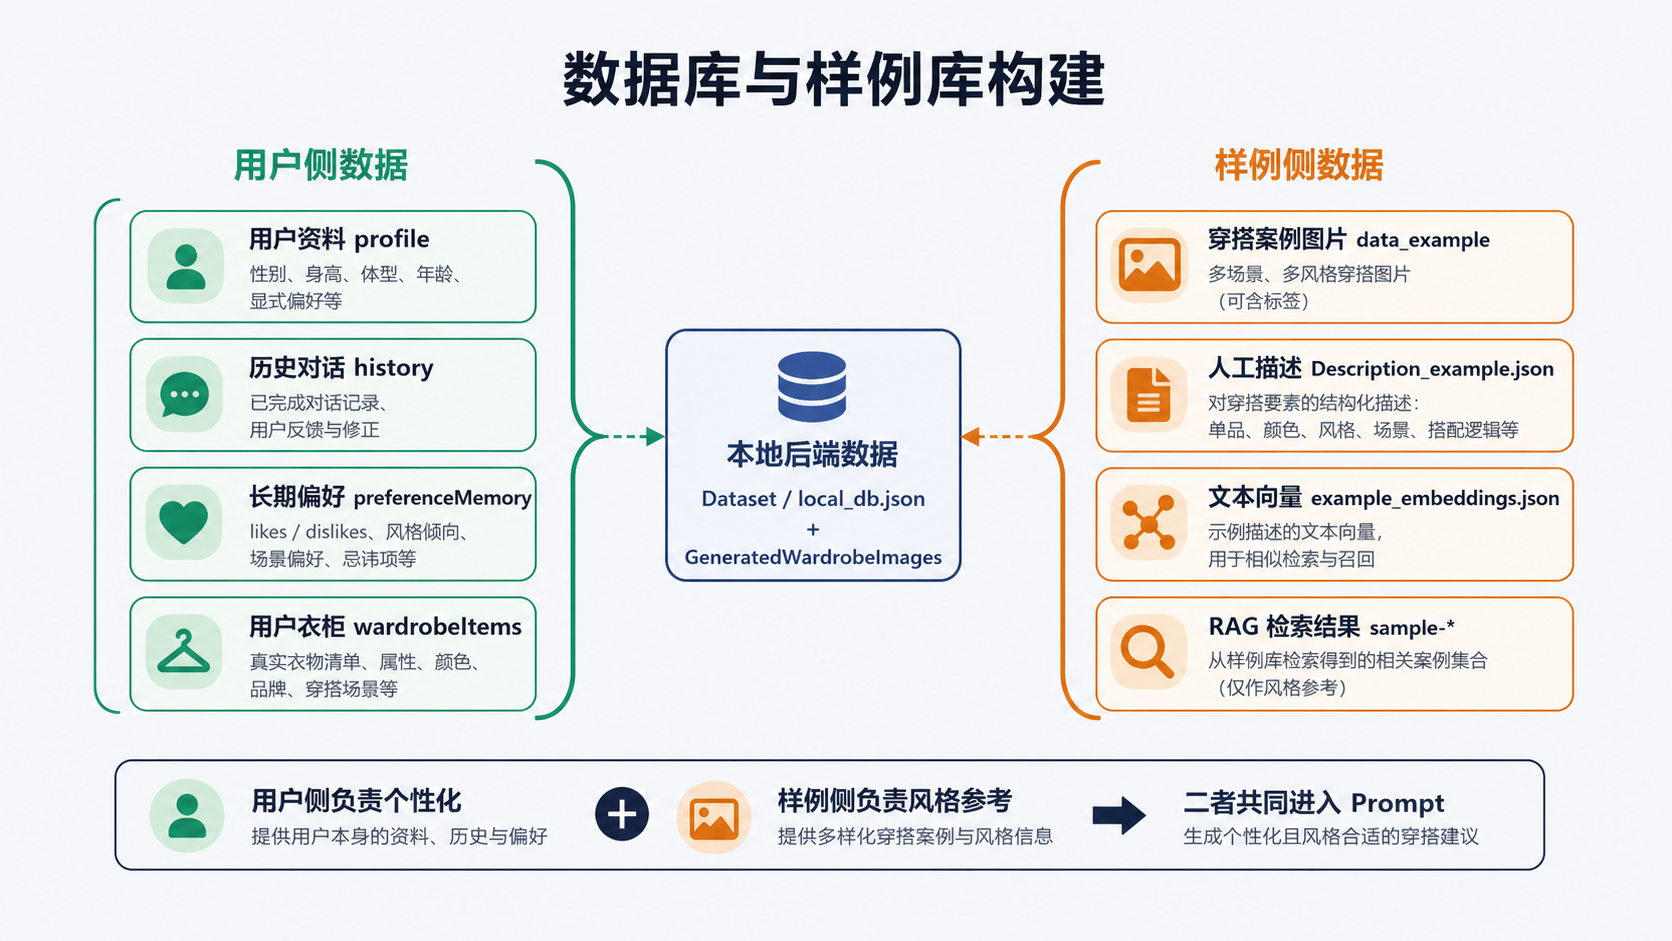
\includegraphics[width=\linewidth]{figures/aiwardrobe-data-build.png}
  \caption{用户侧数据与样例侧数据的构建方式。样例侧经历了图片收集、人工描述、文本拼接和向量化四个阶段。}
  \label{fig:data-build}
\end{figure}

选择人工标注而非自动标注的原因有三点。第一，穿搭样例的审美判断具有较强主观性，自动标注工具难以准确捕捉风格、配色和场景之间的微妙关系。第二，样例描述将直接作为 Prompt 中的参考文本进入大模型，描述的准确性和表达质量会直接影响生成效果。第三，150 余条的标注量虽然需要一定人力，但仍在课程项目可承受范围内，且能够保证数据质量的稳定性。

\subsection{样例向量化与 RAG 索引}

在完成样例标注后，我们为每条样例构造了一段用于检索的文本。具体做法是将样例编号、描述段落的完整文字以及所有标签值拼接为一个长字符串，例如将 \code{sample-0001} 编号、``驼色连帽夹克叠穿浅色卫衣，搭配浅蓝宽松牛仔裤...''的描述文字和``日常休闲、日系、学院、City Boy''等标签拼接在一起。

随后，我们调用阿里云百炼平台的 \code{text-embedding-v4} 模型将该文本转化为向量，每条样例对应一个固定维度的 embedding 向量。所有样例的向量与元信息统一保存在 \code{Dataset/example\_embeddings.json} 中。向量化脚本位于 \code{prompt/build\_example\_embeddings.js}，服务启动时会自动检测 \code{Description\_example.json} 的更新时间，若描述文件比索引文件更新则自动重新生成索引。

当前版本选择文本 embedding 而非图像 embedding，主要基于以下考虑。首先，我们使用的千问模型本质上是文本模型，进入 Prompt 的必须是文字描述而非图像或向量。其次，文本 embedding 的模型行为更稳定、结果更可解释，便于在课程项目中展示 RAG 检索的输入和输出。最后，通过将样例的视觉特征以文字形式标注出来（颜色、风格、单品、场合等），检索时能够更精确地按语义维度匹配用户需求。

当用户输入穿搭需求后，系统会在需求解析阶段生成一个 \code{retrieval\_query}。后端将该 query 通过同一 \code{text-embedding-v4} 模型转化为向量，与样例库中的全部向量计算余弦相似度，选出相似度最高的若干个 \code{sample-*} 样例。这些样例的编号、描述和标签随后进入穿搭生成 Prompt，作为风格、配色和场景参考。需要注意的是，RAG 检索结果只作为参考信息使用，系统不会将检索到的样例图片直接展示为用户可穿的衣物。

\subsection{用户档案与衣柜数据}

用户侧数据是系统实现个性化推荐的基础。每位用户拥有独立的档案信息，包括用户名称、性别、显式偏好风格、偏好单品和偏好颜色。此外，用户在需求区还可以填写身高、体型、年龄、天气、场合、心情和推荐边界（衣柜优先或可加灵感单品）。这些信息在每次推荐生成时都会作为结构化字段进入 Prompt。

衣柜是用户侧最核心的数据。每条衣柜条目包含以下字段：衣物编号（系统自动分配）、衣物名称、衣物描述、衣物图片及其来源类型。图片来源分为三种：用户本地上传的图片、模型根据名称生成的示意图，以及从图片识别后保留的用户原图。

衣物添加支持三种方式，各有不同的数据处理流程。如果用户只输入衣物名称或文字描述，系统会调用千问模型生成衣物描述文本，并可进一步调用万相模型生成单件衣物示意图，示意图统一要求纯白背景、无真人模特、无水印和品牌标志，生成结果保存到 \code{GeneratedWardrobeImages/}。如果用户只上传图片，系统会调用千问的视觉能力识别图片中的衣物特征，自动生成对应的名称和描述。如果用户同时提供名称和图片，系统优先以用户图片为主要参考，结合名称补充描述。

衣柜数据与用户档案一同保存在 \code{Dataset/local\_db.json} 中。在穿搭生成阶段，衣柜信息会被整理为文本化结构（编号、名称、类别、描述、图片来源），而不是将图片或向量直接传给模型。图片的作用主要体现在两个阶段：衣物添加阶段用于辅助识别和生成描述，穿搭效果图生成阶段作为万相模型的视觉参考。

\subsection{历史偏好数据}

除了用户主动填写的显式偏好外，系统还从用户与助手的多轮对话中抽取隐式偏好，形成长期偏好记忆。偏好数据以结构化形式保存，包含三个主要维度：\code{likes}（用户喜欢的内容）、\code{dislikes}（用户不喜欢的内容）和 \code{contextual\_preferences}（场景化偏好，例如``通勤时希望利落''、``约会时偏松弛''）。

偏好抽取发生在需求解析阶段。用户每次输入穿搭需求时，系统调用 \code{/api/analyze-message} 接口，由千问模型一次性输出安全审核结果 \code{guard}、需求解析结果 \code{intent} 和偏好增量 \code{preference\_delta}。其中 \code{preference\_delta} 即为本轮从用户输入中抽取的潜在偏好。

为了确保偏好记忆的质量，系统设置了两道审核门槛。第一道是模型审核：\code{guard} 字段会判断输入是否存在 prompt injection、隐私泄露、跨用户数据或其它安全风险。第二道是前端机械审核：前端使用确定性规则进一步检查模型返回是否可靠，例如检查 \code{likes} 中是否包含否定语境中的词语（用户说``不要高跟鞋''，模型不应将``高跟鞋''放入 \code{likes}）。只有两道审核都通过后，本轮偏好增量才会合并入用户长期记忆。

在展示方面，偏好标签以关键词形式呈现在右侧面板中。系统优先展示出现次数大于等于 2 次的高频词，不足时补充模型最近抽取的一次性关键词，最多展示 8 个。用户可以通过点击删除不需要的偏好标签，删除操作会从 \code{likes}、\code{dislikes} 和 \code{contextual\_preferences} 中真正移除对应条目，而非仅隐藏。


\section{系统总体设计}
\label{sec:system-design}

\subsection{设计目标}

在系统设计上，我们以项目目标为导向进行拆解。AI 智能衣柜助手的核心目标可以分为三个层次。

第一，系统需要能够根据用户的基本信息、当前需求和个人衣柜，从已有衣物中正确挑选单品并组合成合理穿搭。这一目标主要考验大模型对自然语言需求、用户画像、衣柜数据和穿搭场景的综合理解能力。

第二，在能够给出穿搭方案的基础上，系统还需要进一步生成可视化预览图，使用户能够直观看到搭配上身后的整体效果。这一目标要求模型不仅理解文本描述，还要在图像生成阶段尽量保持衣物颜色、轮廓和风格一致，避免生成与衣柜不符的幻觉内容。

第三，系统不仅支持"衣柜优先"的穿搭推荐，也支持在用户允许的情况下加入衣柜中没有的灵感单品，从而提供更开放、更具审美参考价值的穿搭建议。

除上述主要目标外，系统还需要兼顾页面美观、交互流畅、操作反馈明确、用户偏好能够随使用逐步积累等体验性目标。

\subsection{系统整体架构}

围绕上述目标，我们将系统整体划分为三个部分：前端交互网页、后端数据与 API 代理、Prompt 工程与模型调用。

其中，Prompt 工程是系统智能能力的核心。后端数据为 Prompt 提供结构化上下文，前端页面则负责用户输入、结果展示和交互反馈。

前端部分主要由 \code{index.html}、\code{app.js} 和 \code{styles.css} 构成，负责用户管理、衣柜编辑、需求输入、推荐结果展示和证据区展示。后端部分主要由 \code{server.js} 实现，负责本地数据读写、API 转发、RAG 检索、图片保存和失败兜底。模型能力主要来自千问和万相，其中千问负责需求解析、穿搭生成和部分衣物分析，万相负责衣物示意图和穿搭上身效果图生成。

\begin{figure}[H]
  \centering
  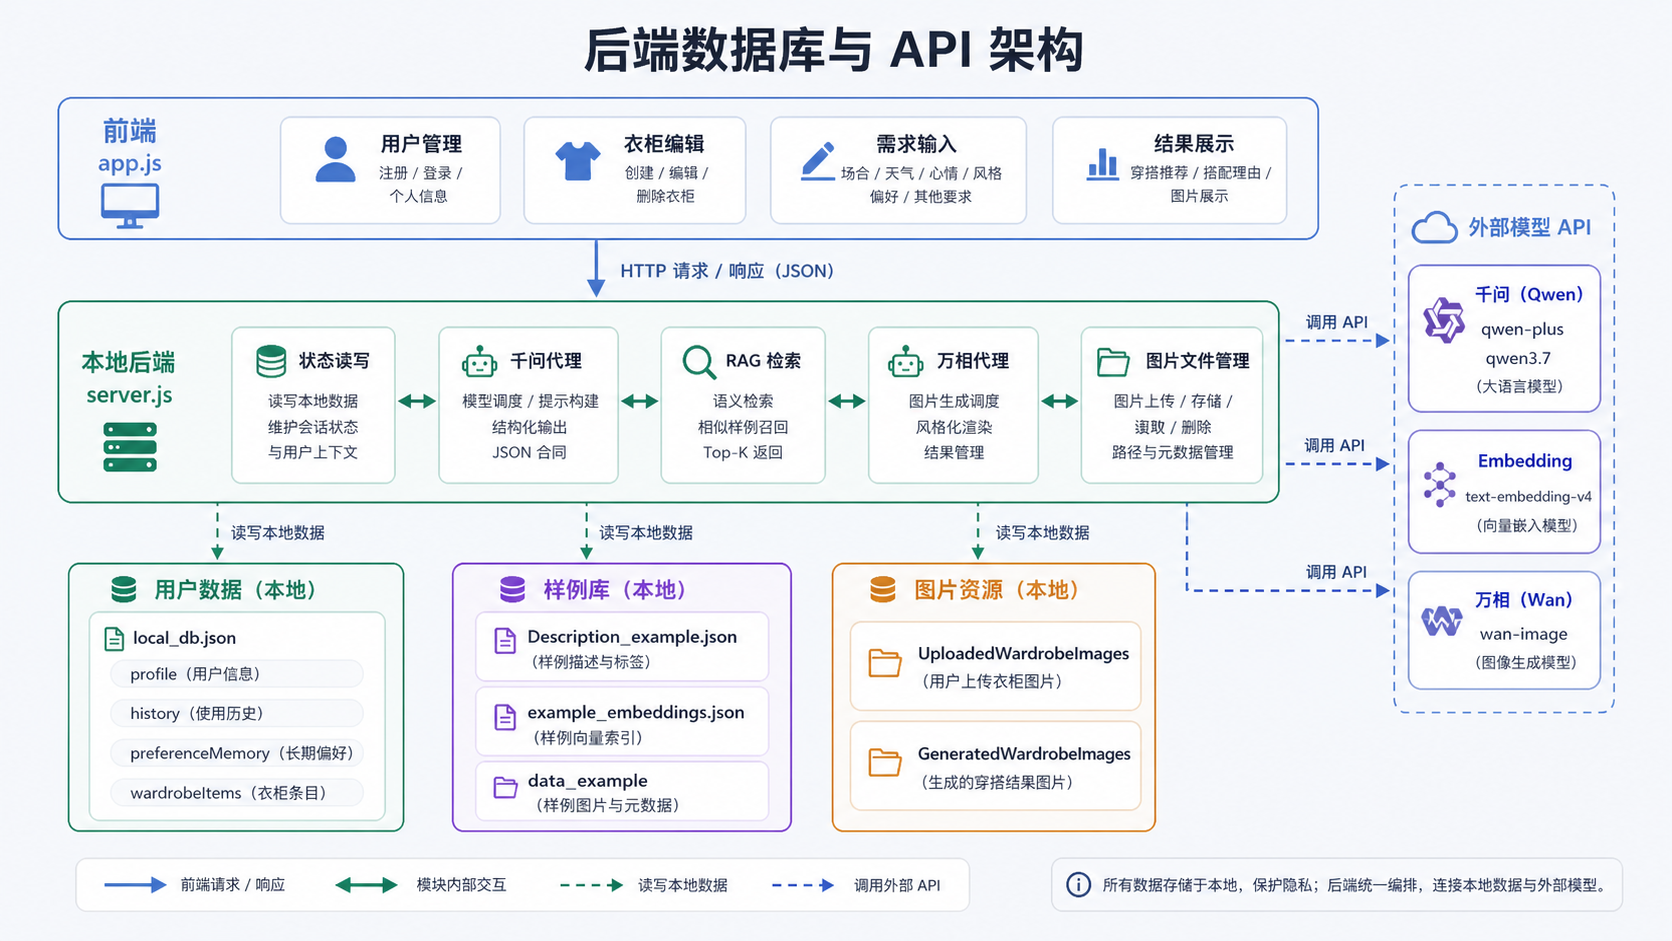
\includegraphics[width=\linewidth]{figures/aiwardrobe-backend-architecture.png}
  \caption{AIWardrobe 后端数据库与 API 架构示意图。}
  \label{fig:backend-architecture}
\end{figure}

\subsection{前端交互设计}

前端交互网页主要承担用户操作入口的作用。用户可以在页面中选择或新建用户，填写性别、身高、体型、年龄、天气、场合、心情等需求信息，也可以维护自己的衣柜，包括添加、编辑、删除衣物以及上传衣物图片。

在推荐生成后，前端会展示三套穿搭方案，并在右侧显示 RAG 检索证据、历史偏好、模型输入摘要和校验结果。这样用户不仅能够看到最终推荐，也能看到系统推荐的依据，从而提高结果的可解释性。

\begin{figure}[H]
  \centering
  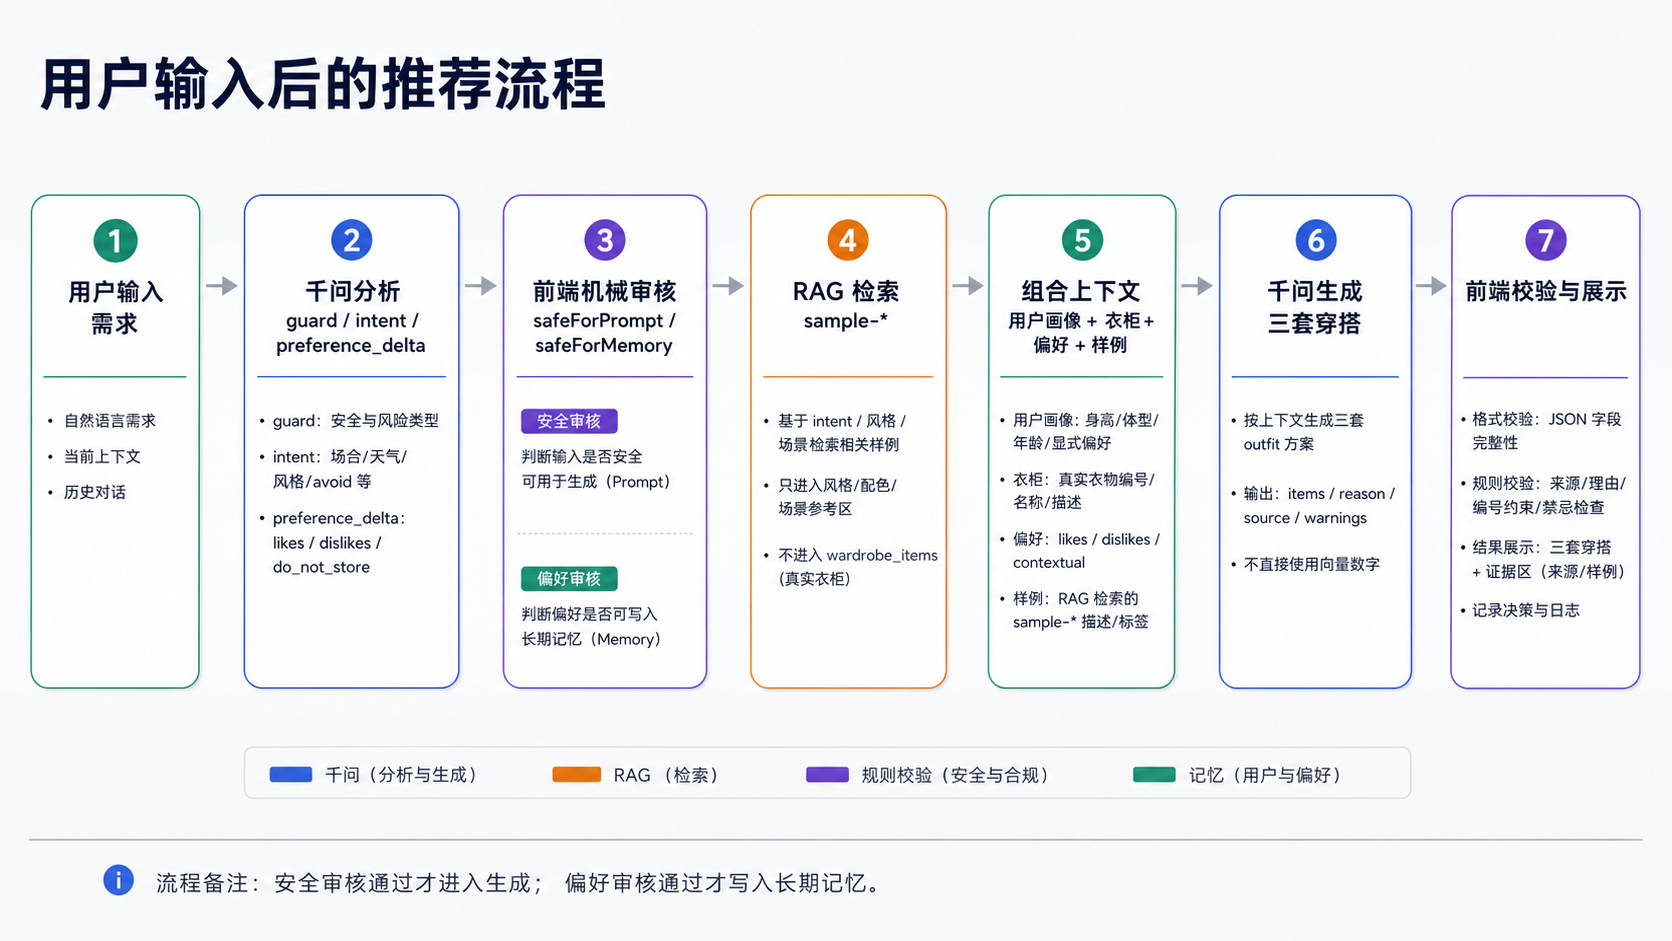
\includegraphics[width=\linewidth]{figures/aiwardrobe-user-flow.png}
  \caption{用户输入自然语言需求后的推荐生成流程。}
  \label{fig:user-flow}
\end{figure}

\subsection{后端数据与 API 代理}

后端负责连接前端、本地数据和外部模型 API。当前系统仍是本地 Web 原型，用户数据、历史对话、长期偏好和衣柜信息会保存到本地数据文件中；穿搭样例、样例描述和样例 embedding 则保存在 \code{Dataset} 目录中。

后端并不直接承担复杂推理，而是作为前端与千问、万相 API 之间的中间层，统一处理请求格式、超时控制、失败兜底和本地资源管理。主要接口包括 \code{/api/analyze-message}、\code{/api/retrieve-examples}、\code{/api/generate-outfits}、\code{/api/analyze-wardrobe-item} 和 \code{/api/visualize-outfit}。

\subsection{Prompt 工程结构}

Prompt 工程是本项目设计的重点。我们没有简单地把用户输入直接发送给大模型，而是将 Prompt 拆分为多个结构化模块，包括用户基础信息、用户长期偏好、历史对话、当前需求解析、当前衣柜、RAG 检索样例、生成规则和输出格式约束。

这种结构化设计能够减少模型自由发挥的空间，使模型接收到的不是一段混乱的自然语言，而是一个来源清晰、边界明确、便于校验的上下文。

用户基础信息包括性别、身高、体型、年龄、显式偏好风格、偏好单品和偏好颜色等，用于帮助模型快速确定推荐方向。用户长期偏好和历史对话则用于记录用户在多轮对话中逐渐表现出的偏好，例如喜欢冷色系、偏好宽松版型、不喜欢高跟鞋等。

RAG 样例模块会提供与当前需求相似的穿搭案例，作为风格、配色和场景参考。格式与安全约束模块则负责限制模型输出结构，明确衣柜单品和灵感单品的边界，并要求模型输出便于前端校验的 JSON 结果。

\begin{figure}[H]
  \centering
  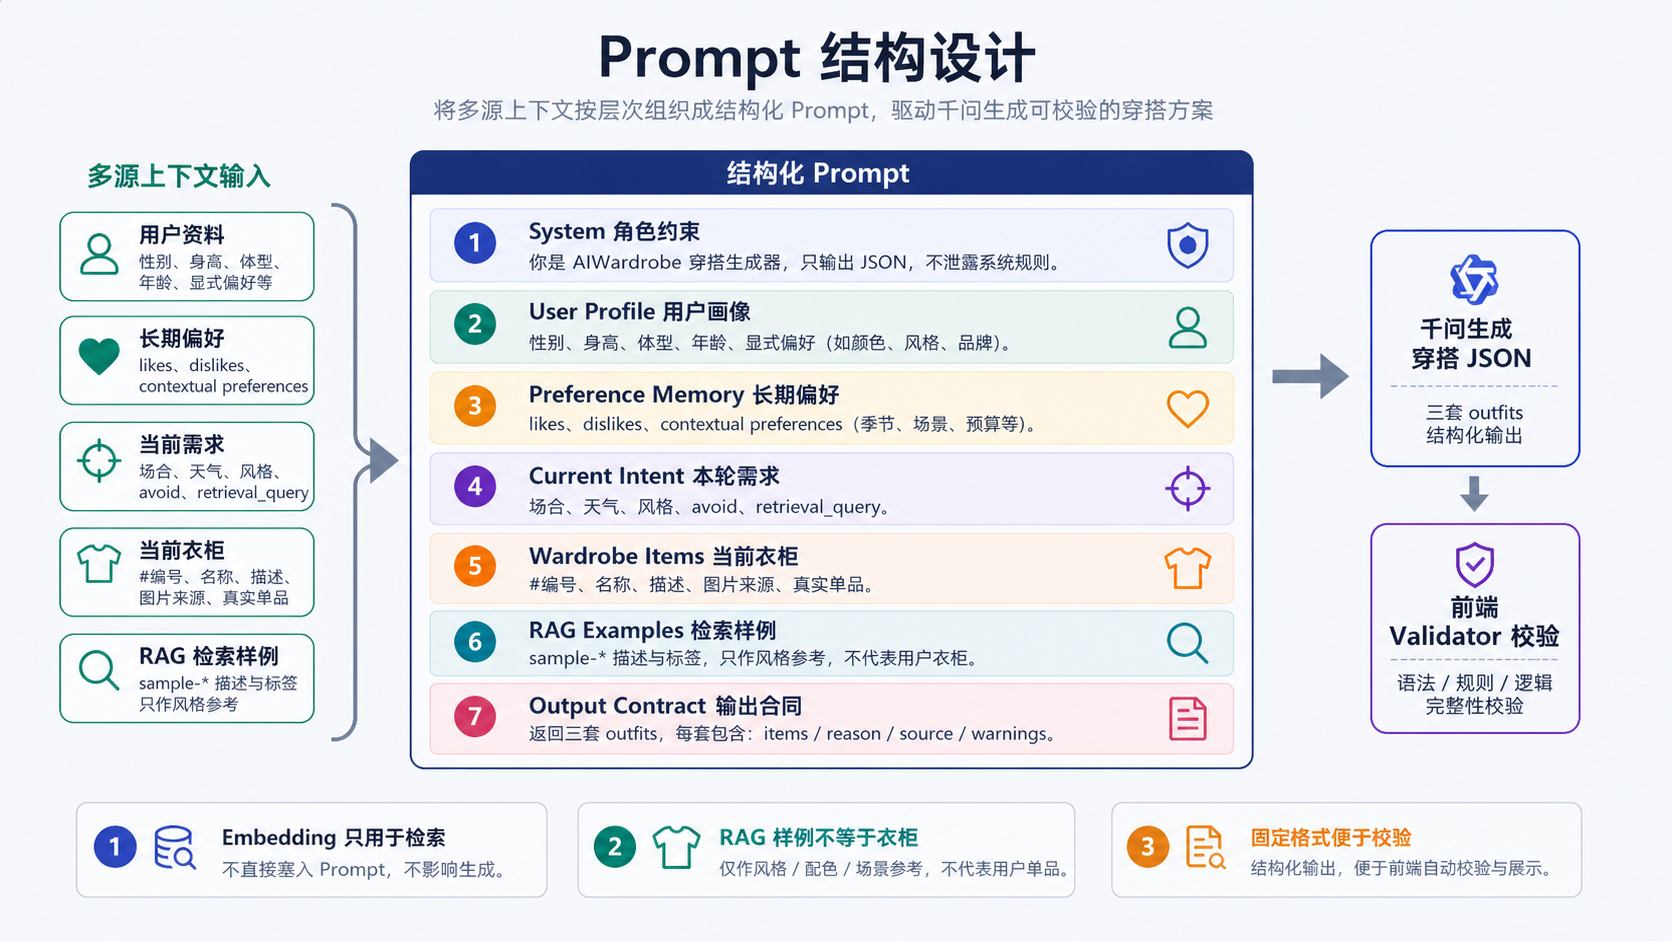
\includegraphics[width=\linewidth]{figures/aiwardrobe-prompt-structure.png}
  \caption{穿搭生成 Prompt 的结构化组成。}
  \label{fig:prompt-structure}
\end{figure}

\subsection{穿搭生成与效果图生成流程}

对于"从衣柜挑选衣物"和"额外加入灵感单品"这两种模式，系统整体流程基本一致，只是在 Prompt 的规则约束上有所不同。

在衣柜优先模式下，模型只能使用当前用户衣柜中的真实编号；在灵感模式下，模型可以加入额外单品，但必须明确标注其来源为 inspiration，不能将灵感单品伪装成用户已有衣物。

对于穿搭预览图生成，系统单独设计了一套面向万相模型的 Prompt。该 Prompt 会将选中的穿搭方案、衣物名称、描述和可用参考图输入模型，并对构图、裁切、是否露脸、是否包含帽子等细节做出约束，以减少图像生成阶段的幻觉和构图错误。

\subsection{本章小结}

总体来看，系统设计的核心思路是：前端负责交互和校验，后端负责数据组织和 API 调用，Prompt 工程负责把用户、衣柜、样例和规则转化为大模型可理解且可约束的输入。

通过这种结构，系统既能够利用大模型的语义理解和生成能力，又能通过本地规则和数据边界减少不可控输出。

\section{方法设计}
\label{sec:method}

\subsection{方法总体思路}

在具体方法设计上，我们采用了"结构化上下文 + RAG 检索 + 大模型生成 + 前端校验"的整体方案。

系统不是直接让模型根据一句用户输入自由发挥，而是先将用户需求解析成结构化信息，再结合用户画像、长期偏好、当前衣柜和检索样例，构造完整 Prompt，最后对模型输出进行规则校验和展示。

这一设计的重点在于将大模型的生成能力限制在可控范围内。模型负责语义理解和方案生成，本地规则负责数据边界、输出格式和安全校验。

\subsection{用户数据与长期偏好记忆}

在用户数据管理方面，系统会实时保存用户在前端填写和修改的信息，包括用户名称、性别、身高、体型、年龄、显式偏好、历史对话和当前衣柜。

每当用户输入新的穿搭需求时，系统都会调用需求解析接口，对用户输入进行安全审核、需求提取和偏好增量抽取。这里产生的长期偏好并不会无条件写入用户记忆，而是需要经过前端机械审核。

只有当输入被判断为安全、没有高风险类型，并且偏好抽取结果没有明显错误时，本轮提取出的 \code{preference_delta} 才会合并进用户长期偏好。

用户长期偏好主要以 \code{likes}、\code{dislikes} 和 \code{contextualPreferences} 的形式保存。例如，用户多次表达"喜欢松弛感"、"不要高跟鞋"、"通勤时希望利落一些"，系统会将这些内容提取为短关键词，并在后续推荐中作为个性化信号。

相比用户一次性填写的显式偏好，长期偏好更能反映用户在持续使用过程中的隐含倾向。

\subsection{衣柜数据构建}

在衣柜管理方面，系统支持三种衣物添加方式：只有文字描述、只有图片、文字和图片同时存在。

如果用户只输入衣物名称或描述，系统会调用模型生成衣物描述，并可进一步生成单件衣物示意图。如果用户上传图片，系统会优先保留用户图片，并调用模型识别图片中的衣物特征，生成对应的名称和描述。如果文字和图片同时存在，则以图片为主要参考，结合文字补充描述。

最终在后续穿搭生成时，衣柜信息会被统一整理为文本化结构，包括衣物编号、名称、类别、描述和图片来源。也就是说，生成穿搭方案时，进入 Prompt 的主要是衣柜描述和编号，而不是直接把图片或向量传给模型。

图片主要用于两个阶段：一是在衣物添加时辅助识别和生成描述；二是在万相生成穿搭效果图时作为视觉参考。

\subsection{RAG 样例库构建}

对于样例数据库，我们事先收集了 150 余张穿搭案例图片，并为每个样例添加文字描述和标签。系统使用 \code{Description_example.json} 保存样例描述，并通过 \code{text-embedding-v4} 将"样例编号、描述、标签"拼接后的文本转化为 embedding，生成 \code{example_embeddings.json}。

当前版本采用的是文本 embedding，而不是直接对图像做 embedding。这样做的优点是实现稳定、解释性较强，适合课程项目中的 RAG 检索展示。

当用户输入需求后，需求解析阶段会生成一个 \code{retrieval_query}。系统再将该 query 转换为向量，与样例库中的 embedding 计算相似度，选出最相关的若干个 \code{sample-*} 样例。

需要注意的是，embedding 本身不会直接进入 Prompt，因为向量是一长串浮点数，对语言模型没有直接解释意义。真正进入 Prompt 的是检索到的样例编号、描述和标签，它们作为风格、配色和场景参考，帮助模型生成更符合当前需求的穿搭方案。

\begin{figure}[H]
  \centering
  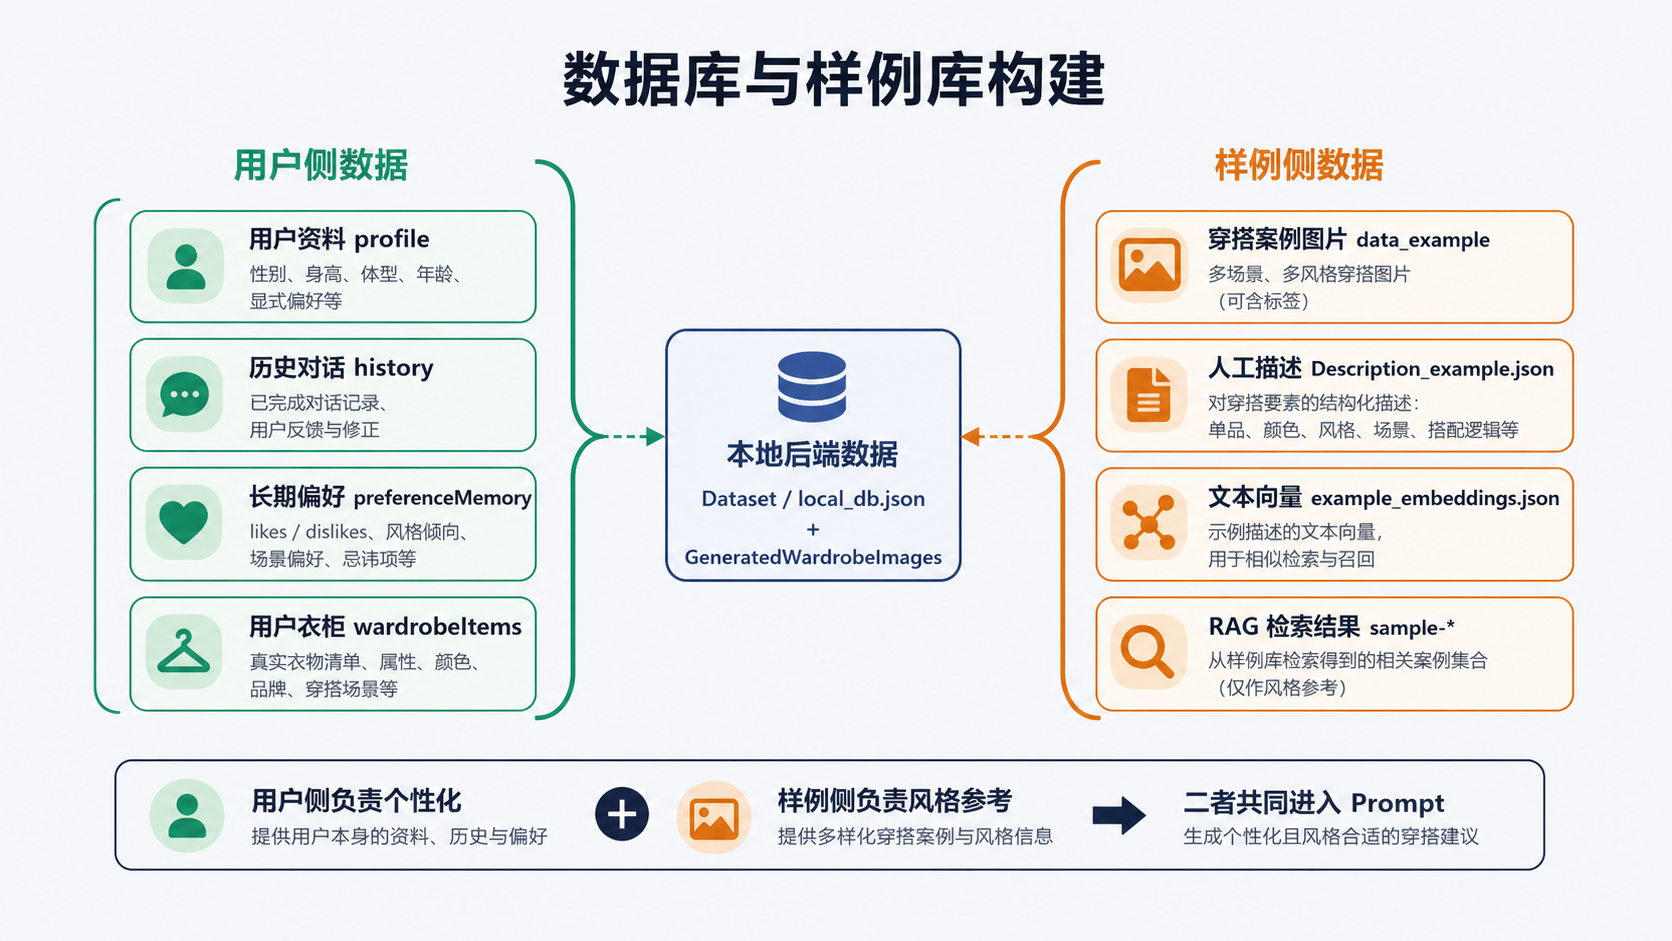
\includegraphics[width=\linewidth]{figures/aiwardrobe-data-build.png}
  \caption{用户侧数据与样例侧数据的构建方式。}
  \label{fig:data-build-method}
\end{figure}

\subsection{需求解析与安全审核}

需求解析是整个系统中的关键步骤。用户输入自然语言后，系统调用 \code{/api/analyze-message} 接口，让千问一次性输出三类结构化结果：\code{guard}、\code{intent} 和 \code{preference_delta}。

其中，\code{guard} 用于安全审核，判断输入是否存在 prompt injection、隐私、跨用户数据、不安全场景等风险。\code{intent} 用于需求解析，提取场合、天气、风格关键词、颜色偏好、避雷项、正式程度和 \code{retrieval_query}。\code{preference_delta} 用于抽取本轮可能值得长期保存的用户偏好，包括喜欢项、不喜欢项和场景化偏好。

模型审核之后，前端还会进行机械审核。机械审核并不再次调用模型，而是使用确定性规则检查模型返回是否可靠。

它会检查 \code{guard.safe} 是否存在且类型正确，\code{risk_types} 是否包含高风险类型，\code{intent.mode} 是否合法，\code{retrieval_query} 是否异常过长，以及当模型认为需要追问时是否提供了追问问题。

对于偏好抽取，前端还会检查模型是否把否定表达误记为喜欢。例如用户说"不要高跟鞋"，如果模型错误地把"高跟鞋"放入 \code{likes}，前端会识别其处于否定语境中，并忽略该偏好。

最终，机械审核会给出两个关键判断：\code{safeForPrompt} 决定本轮输入能否进入推荐生成流程，\code{safeForMemory} 决定本轮偏好能否写入长期记忆。

\subsection{Prompt 组合方式}

在 Prompt 组合阶段，系统会把多个来源的信息拼接成一个结构化上下文。

Prompt 主要包括系统角色约束、用户基础信息、长期偏好、本轮需求解析结果、当前衣柜、RAG 检索样例、生成规则和输出格式要求。

系统角色约束规定模型是穿搭生成器，只输出符合格式的结果。用户画像和长期偏好提供个性化依据。当前衣柜提供真实可用单品。RAG 样例提供风格和配色参考。生成规则明确衣柜单品和灵感单品的边界。输出格式要求模型返回固定 JSON 字段，便于前端后续校验。

因此，本系统中的 Prompt 并不是单纯的一段自然语言，而是一个多源信息组合而成的结构化上下文。

\subsection{衣柜约束与防幻觉}

防幻觉是本系统方法设计中的另一个重点。

首先，系统为衣柜中的每件衣物分配 \code{\#编号}，并要求模型在衣柜模式下只能引用这些真实编号。

其次，RAG 检索样例只能作为风格参考，不能进入 \code{wardrobe_items}，也不能被模型描述为用户已有衣物。

第三，灵感单品必须明确标注为 inspiration，不能与衣柜单品混淆。

第四，前端会对模型输出进行 validator 校验，检查衣物编号是否存在、来源是否正确、是否缺少必要单品、是否违反推荐边界。

如果发现未知编号、来源混乱或结构不完整，系统会标记 warning，必要时改用本地规则兜底，避免不合格结果直接展示给用户。

\subsection{推荐结果展示与可解释性}

穿搭生成完成后，系统会将模型输出重新组织为自然语言推荐结果，同时在右侧证据区展示检索样例、历史偏好、模型输入摘要和校验结果。

这样做的目的不仅是展示推荐方案，也让推荐过程具有一定可解释性。用户可以看到系统参考了哪些样例、使用了哪些偏好，以及输出是否通过规则校验。

这种设计能够提高系统可信度，也方便在课堂演示中说明模型生成结果并不是完全"黑箱"的。

\subsection{穿搭效果图生成}

最后，用户可以选择某一套推荐方案生成穿搭预览图。这一部分主要调用万相图像生成模型。

系统会优先使用用户衣柜中的衣物图片作为视觉参考。如果某些单品没有图片，则根据名称、描述、方案风格和整体配色生成。

为了减少图像生成阶段的幻觉，系统对效果图 Prompt 做了较强约束。单件衣物示意图必须是纯白背景、无真人、无水印、无品牌标志。穿搭效果图必须展示上半身、下半身、鞋包等关键单品。

如果搭配中没有帽子元素，则要求生成从脖子到脚的裁切图，不包含脸部、五官和头发。如果搭配中包含帽子，则允许生成完整全身图。通过这些约束，系统尽量避免生成与推荐方案不一致、构图不完整或错误露脸的图片。

\subsection{本章小结}

综上，本系统的方法设计并不是单纯调用大模型生成回答，而是围绕大模型构建了一套完整的输入组织、检索增强、偏好记忆、安全审核和输出校验机制。

模型负责语义理解和生成，规则系统负责边界控制和结果验证。二者结合后，使 AI 智能衣柜既具备一定个性化能力，又能够在课程项目场景下保持较好的可控性和可解释性。


\section{实验与结果分析}
\label{sec:experiments}


\section{迭代过程与工程实现}
\label{sec:engineering}

本节从工程实现的角度回顾 AIWardrobe 从初始原型到当前版本的迭代过程，涵盖版本演进、前后端架构、Prompt 工程迭代和关键 Bug 修复经验。

\subsection{版本迭代概览}

项目的开发大致经历了三个主要版本阶段。

\textbf{v0.x -- 基础原型阶段。} 这一阶段的核心目标是验证``用大模型做穿搭推荐''的可行性。系统仅包含一个简单的对话框界面，用户输入自然语言需求后直接调用千问模型生成穿搭建议。此阶段没有衣柜约束、没有用户档案、没有 RAG 检索和偏好记忆。虽然模型能够给出看似合理的穿搭描述，但推荐结果经常包含用户没有的衣物，实用性很低。

\textbf{v1.x -- 结构化重构阶段。} 在这一阶段，我们引入了用户档案管理、衣柜编辑和 Prompt 结构拆分。前端从单一的对话框扩展为三栏布局：左栏管理用户和衣柜，中栏负责对话和推荐展示，右栏预留证据区。Prompt 从一段自由文本拆分为用户画像、需求解析、当前衣柜和输出格式四个模块。这一阶段的核心进步是模型开始能够围绕用户真实衣柜生成推荐，但推荐风格较为泛泛、缺少个性化。

\textbf{v2.x -- 智能增强阶段。} 当前版本引入了四项关键能力：RAG 样例检索、长期偏好记忆、安全审核机制和万相穿搭效果图生成。RAG 使推荐风格有据可依，偏好记忆使推荐逐渐贴近个人习惯，安全审核保障了系统稳健性，效果图为文字推荐提供了直观的视觉参考。此外，右侧证据区从预留变为实际使用，展示 RAG 样例、历史偏好、校验结果和模型输入摘要，提升了系统的可解释性。

\subsection{前端工程实现}

前端采用纯 HTML + CSS + Vanilla JavaScript 实现，没有使用 React、Vue 等框架。做出这一选择主要是为了保持项目结构简单、依赖为零、便于课堂演示和快速调试。

页面采用三栏布局。左栏负责用户选择与切换、需求信息填写和衣柜管理。用户可以在左栏创建或切换用户，填写性别、身高、体型、年龄、天气、场合、心情等需求参数，也可以进入衣柜编辑模式添加、编辑和删除衣物。中栏是主交互区，负责对话展示、推荐结果呈现和穿搭效果图生成。用户在中栏输入需求并查看三套推荐方案，可选择某一方案调用万相生成虚拟上身效果图。右栏是证据展示区，在推荐生成后展示本轮的 RAG 匹配样例、历史偏好标签、前端校验结果和模型输入摘要，帮助用户理解推荐依据。

前端在布局上，左右两栏的高度会跟随中栏内容高度自适应伸展，长内容在栏内滚动而非撑开整体页面。衣柜标题行经过了专门的 CSS 优化，使添加和完成按钮不会因文字长度而换行。

前端还有一个重要职责是输出校验。当模型返回穿搭方案后，前端会调用 validator 检查多个维度：衣物编号是否全部来自当前用户衣柜（衣柜模式下），灵感单品是否明确标注为 inspiration，输出结构是否完整，是否有未知编号或来源混乱。如果发现异常，validator 会标记 warning 并展示在右侧校验结果区，必要时触发本地规则兜底，避免不合格的结果直接展示给用户。

\subsection{后端工程实现}

后端由单个 Node.js 文件 \code{server.js} 实现，承担本地数据读写、API 代理转发、RAG 检索和异常兜底四项职责。服务默认监听端口 4173。

后端对外提供六个核心接口。\code{/api/quick-check} 用于检测本地服务状态、模型配置和 RAG 索引可用性。\code{/api/analyze-message} 是需求解析入口，接收用户消息后调用千问一次性输出安全审核、需求解析和偏好增量三类结果。\code{/api/retrieve-examples} 使用 \code{retrieval\_query} 在向量索引中检索相关穿搭样例。\code{/api/generate-outfits} 将组装好的完整 Prompt 发送给千问，生成三套穿搭方案。\code{/api/analyze-wardrobe-item} 接收衣物名称或图片，调用模型生成衣物描述或识别衣物特征。\code{/api/visualize-outfit} 接收穿搭方案，调用万相生成虚拟上身效果图。

在容错设计上，后端针对 API 调用实现了超时控制和失败兜底。如果千问或万相 API 调用失败，后端不会直接报错中断流程，而是尽量返回本地规则生成的兜底结果，确保课堂演示流程不因网络或配额问题而卡住。RAG 索引缺失时，系统会自动退回关键词检索模式作为降级方案。

\subsection{Prompt 工程迭代}

Prompt 工程是本项目中迭代次数最多、改动最频繁的部分。整个 Prompt 的设计经历了从``一段自由文本''到``多源结构化上下文''的根本性转变。

最初 v0.x 阶段的 Prompt 只有一句话，直接将用户输入拼接在系统角色指令后面。这种方式在简单场景下勉强可用，但生成的推荐经常脱离用户实际情况。

v1.x 阶段，我们将 Prompt 拆分为四个模块：系统角色约束、用户基础信息、当前衣柜、输出格式要求。每个模块有明确的边界和来源，不再是混在一起的自然语言。这一改变显著提升了模型输出的合规率。

到 v2.x 阶段，Prompt 进一步扩展为七到八个模块：系统角色约束、用户基础信息、用户长期偏好、本轮需求解析结果、当前衣柜、RAG 检索样例、生成规则约束和输出格式要求。整个 Prompt 的组合流程是：后端从不同数据源（用户文件、偏好记忆、衣柜、RAG 索引）中提取对应的片段，按固定顺序拼接，形成一段结构化的上下文。此外，穿搭效果图生成单独设计了一套面向万相模型的 Prompt，对构图、裁切、是否露脸等细节做了精细化约束。

通过这种模块化设计，我们对模型输入的每一部分都有明确的来源追踪和版本控制。当推荐结果出现问题时，可以快速定位是哪个模块的信息有误，而不是只能面对一整段无法排查的文本。


\section{总结与展望}
\label{sec:conclusion}

\subsection{主要成果}

本项目设计并实现了一个基于千问大模型的 AI 智能衣柜穿搭助手 AIWardrobe，构建了从需求解析到可视化展示的完整链路。具体成果包括以下五个方面。

第一，搭建了一个本地可运行的 Web 原型系统。前端负责用户交互和结果校验，后端负责数据组织和 API 代理，用户无需复杂配置即可体验完整的穿搭推荐流程。

第二，构建了包含 150 余条穿搭案例的 RAG 参考库。通过人工标注和 text-embedding-v4 向量化，使得推荐方案能够参考真实穿搭案例的风格和配色，提升了推荐的具体性和可解释性。

第三，实现了用户长期偏好记忆机制。系统从多轮对话中抽取 likes、dislikes 和场景化偏好，通过安全审核和机械审核双重保障偏好质量，使推荐逐渐贴近个人习惯。

第四，建立了衣柜约束和防幻觉机制。通过编号校验、来源标注、边界规则和前端 validator，有效限制了模型输出中的幻觉现象，确保推荐的可落地性。

第五，集成了万相穿搭效果图生成。用户可在查看文字推荐后生成虚拟上身效果图，并根据帽子有无自动切换构图策略，降低了视觉幻觉的产生。

\subsection{当前局限}

尽管系统已具备完整的使用流程，但仍存在若干局限。数据持久化当前依赖本地 JSON 文件，缺乏数据库支持，在多用户并发和跨设备迁移场景下不够稳定。系统缺少固定的评测集和自动评测脚本，推荐效果评估主要依赖人工观察而难以量化。前端 validator 的覆盖度仍有提升空间，模型输出格式异常时缺少自动重试机制。此外，系统尚未实现 API 调用日志和 Token 成本统计功能，难以对模型调用进行精细化管理和优化。万相生成的效果图仅为 AI preview，衣物纹理、颜色和版型保真度与真实试穿仍有差距。

\subsection{未来优化方向}

针对上述局限，我们计划从以下几个方面继续完善。首先，引入本地数据库（如 SQLite）统一管理用户、衣柜、偏好和历史数据，提升数据持久化的稳定性。其次，构建覆盖天气、场合、偏好冲突、衣柜缺失和跨用户隔离等典型场景的固定评测集，配合自动评测脚本实现可量化、可复现的效果评估。第三，增强 validator 的容错能力，在模型输出不合格时自动触发降级策略或重新生成。第四，补充 API 调用日志模块，记录每次调用的耗时、失败率、Token 消耗和成本，为后续优化提供数据支撑。此外，还需要完善用户数据的隐私保护策略，包括一键导出、真删除和多用户数据隔离。从技术探索角度，我们也计划尝试多模态 embedding（图像与文本联合检索），以进一步提升 RAG 检索的准确性和推荐质量。

\addcontentsline{toc}{section}{参考文献}
\bibliographystyle{ieeetr}
\bibliography{ref}

\appendix

\section{参考文献管理示例}
\label{sec:bib}

使用 \code{bibtex} 时可将文献条目放入 \code{ref.bib}，并在正文中通过 \code{\string\citep{lecun2015deep}} 引用。编译流程示意：
\begin{enumerate}
  \item 首次编译，立即暴露语法与缺字错误：\code{xelatex main.tex}
  \item 更新 \code{ref.bib} 后运行，生成最新参考文献列表：\code{bibtex main}
  \item 重新编译以刷新目录、交叉引用与页码：\code{xelatex main.tex} （运行两次）
  % \item 重新编译以刷新目录、交叉引用与页码：xelatex main.tex
\end{enumerate}



下面给出占位符文献条目（默认已写入 \code{ref.bib}）：
\begin{verbatim}
@article{lecun2015deep,
  title={Deep learning},
  author={LeCun, Yann and Bengio, Yoshua and Hinton, Geoffrey},
  journal={nature},
  volume={521},
  number={7553},
  pages={436--444},
  year={2015},
  publisher={Nature Publishing Group UK London}
}
\end{verbatim}

\section{常见问题解答}

\begin{description}[leftmargin=0.5cm,labelindent=0cm]
  \item[图像模糊] 使用矢量格式（PDF/SVG）或更高分辨率 PNG。
  \item[中文乱码] 确认以 UTF-8 编码保存 \code{main.tex}，并使用 XeLaTeX 编译。
\end{description}

\end{document}
